
%%%%%%%%%%%%%%%%%%%%%%% file typeinst.tex %%%%%%%%%%%%%%%%%%%%%%%%%
%
% This is the LaTeX source for the instructions to authors using
% the LaTeX document class 'llncs.cls' for contributions to
% the Lecture Notes in Computer Sciences series.
% http://www.springer.com/lncs       Springer Heidelberg 2006/05/04
%
% It may be used as a template for your own input - copy it
% to a new file with a new name and use it as the basis
% for your article.
%
% NB: the document class 'llncs' has its own and detailed documentation, see
% ftp://ftp.springer.de/data/pubftp/pub/tex/latex/llncs/latex2e/llncsdoc.pdf
%
%1.rauch2011mobile
%2.gunduz2012usability
%3.hussain2008user
%4.martinazzo2008testing
%5.nayebi2012state
%6.seraj2012study
%7.kondratova2006m
%8.lee2004developing
%9.hashim2011mobile
%%%%%%%%%%%%%%%%%%%%%%%%%%%%%%%%%%%%%%%%%%%%%%%%%%%%%%%%%%%%%%%%%%%


\documentclass[runningheads,a4paper]{llncs}


\usepackage{url}
\usepackage{paralist}
\usepackage{cite}
\usepackage[numbers]{natbib}
\usepackage{graphicx}
\graphicspath{ {images/} }

\urldef{\mailsa}\path|{firstname.lastname}@deri.ie|
\usepackage{listings}
\usepackage{color}

\definecolor{dkgreen}{rgb}{0,0.6,0}
\definecolor{gray}{rgb}{0.5,0.5,0.5}
\definecolor{mauve}{rgb}{0.58,0,0.82}

\lstset{frame=tb,
  language=Java,
  aboveskip=3mm,
  belowskip=3mm,
  showstringspaces=false,
  columns=flexible,
  basicstyle={\small\ttfamily},
  numbers=none,
  numberstyle=\tiny\color{gray},
  keywordstyle=\color{blue},
  commentstyle=\color{dkgreen},
  stringstyle=\color{mauve},
  breaklines=true,
  breakatwhitespace=true,
  tabsize=3
}

\begin{document}

\mainmatter  % start of an individual contribution

\begin{titlepage}

\begin{center}
\Huge{\textsc{Combating Screen Size Limitations by Developing a Universal Application}} \\
\vspace{4em}
\large{Dissertation Submitted To} \\
Damien Costello \\
\vspace{2em}
\Large{\textsc{Galway-Mayo Institute Of Technology}} \\
\vspace{1em}
\large{in partial fulfilment of the requirements} \\
\large{of the award of the degree} \\
\vspace{2em}
\Large{\textsc{Bachelor Of Science (Honours) In Software Development}} \\
\vspace{2em}
by \\
\vspace{1em}
\textbf{\textsc{Majella Greene}} \\
\vspace{4em}
\Large{\textsc{School of Science}} \\
\Large{\textsc{Galway-Mayo Institute of Technology}} \\
\Large{28th May 2015}
\end{center}
\vspace*{\stretch{1}}
\end{titlepage}
\newpage\setcounter{tocdepth}{2}
\tableofcontents\newpage


\begin{abstract}
In this paper, we examine the design and usability of mobile device applications. The main functionalities and user experience are crucial in mobile applications being successful. As mobile devices have small screens, this hinders mobile usability as it causes limitations for the amount of data that can be viewed by the user at one time. This problem can be overcome by developing a Windows 8.1 universal application which would eliminate the screen size limitations as it can be viewed on a bigger screen(Tablet, Desktop etc). The mobile phone version of Crystal Clear will show less data than the tablet version but will still show the critical parts of the application. This is one main factor that will enhance user's experience and will eliminate the small screen restrictions.
\end{abstract}

\keywords 
Multimodal interaction, Speech Technology, VoiceXML
\section{Introduction}
\subsection{Several Problem Statements}
\begin{inparaenum}[]
{\texttt{"Visualization can make a wide range of mobile applications more intuitive and productive. The mobility context and technical limitations such as small screen size make it impossible to simply port visualization applications from desktop computers to mobile devices, but researchers are starting to address these challenges"\cite {seraj2012study}}} 
\end{inparaenum}

\begin{inparaenum}[]
Visual tools have been relied on for understanding problems which solve the issues in less time (eg. maps, diagrams and charts). Incorporating these tools into this Windows 8.1 universal application will enhance the usability of the application. The wide range of improvements in computers' graphic capabilities and processing power has allowed computing application domains to incorporate advanced visualization techniques. Incorporating these capabilities to mobile phones could address complex visualization problems. Nevertheless, the technical restrictions of the small screen make it possible to do the simple task of porting applications from desktop computers to mobile phones.
\end{inparaenum}

\begin{inparaenum}[]
The user's view of the textual information is limited on the screen of a mobile device. This may cause the user to become frustrated with using a mobile device compared to the ease of reading information on a desktop computer screen. All mobile devices have their own unique usability obstacles. By limiting the data on the mobile phone version of the application, this will alleviate potential problems. Crystal Clear, a Windows 8.1 universal application is proposed to be be developed. The overall vision of this universal application is to give the user a useful application for their everyday life. It will give the user the opportunity to calculate their water bill to see how much water they are using and estimate how much it will cost. It is envisaged that this application will be a huge advantage to anyone trying to budget. When the water meter bills were introduced earlier this year, there were alot of objections. This was primarily due to the fact that the population of Ireland would be paying for a resource that had previously been free. This left a huge gap in the Windows 8.1 market for an application like Crystal Clear.
\end{inparaenum}

\subsection{Objectives and Aims}
\begin{inparaenum}[]
There are several meter reading applications (electricity, oil etc.) on the Apple and Android market, however there has been no particular application for water meters on the Windows 8.1 market. Such applications as water conservation information applications are already present on the Windows 8.1 store but no particular effort has been made to calculate a water bill from meter readings being inputted by the user. The main aim of Crystal Clear is to develop a universal Windows 8.1 application to keep track and record all water usage in the home. This can be implemented by taking a reading from your water meter and inputting that reading of the daily litres used  into the application. The inputted data will be saved into longterm storage to compare and predict your future water bills.
\end{inparaenum}

\begin{inparaenum}[]
The main reason for this is that all Irish households have to pay for their water usage since earlier this year. Also, it is hoped that this application would be a leader in customer service to ensure people are saving money on their water bills and have awareness to where there money is going. There is a huge niche in the market for this application due to increasing costs for household owners. 
\end{inparaenum}

\section{Literature Review}
\begin{inparaenum}[]
\subsection{Introduction}
{\texttt{Mobile Usability}} is an ease of use and functionalities of a mobile application. It plays a predominant role in the users overall experience in using any software product. In mobile applications, usability is crucial. The user wants an enjoyable, easy to use design pattern. Therefore, usability considerations must be applied when developing and designing mobile applications.
\cite{martinazzo2008testing}

 Usability is known as
\it"The effectiveness, efficiency and satisfaction with which specified users can achieve specified goals in particular environments"\cite{gunduz2012usability}
\rm Whereas user experience defines
\it "A person's perceptions and responses that result from the use or anticipated use of a product, system or service".\cite{gunduz2012usability}

\rm The progression and evolution of mobile devices in later years have expanded dramatically compared to a device that would dial numbers to contact a personal digital assistant (PDA). Mobile devices with applications have increased in popularity and are now the standard for consumers when it comes to devices. 
\cite{lee2004developing}
\end{inparaenum}

\begin{inparaenum}[]

\end{inparaenum}
In this paper, we examine the specification of mobile usability and the main concerns of mobile usability when developing applications. By examining these papers one can compare and contrast the views of these authors on their opinion of mobile usability.
 

\subsection{Issues in Mobile Usabilty}
\label{sec:Issues in Mobile Usabilty}
There are key differences between a mobile device and a desktop computer and these differences in usability must be addressed. All mobile devices have their own unique usability obstacles. \citet{rauch2011mobile} noted that these obstacles include download delays, small screens, poor resolution and difficult mechanisms for user input, and mostly typing . 
Portability is a unique issue and is key for the device as it will be taken around with the user in their pocket or bag. 
Reading on a mobile device has its disadvantages compared to reading on a desktop computer, as it is difficult to appreciate the content when reading it on a small screen.
\begin{inparaenum}[]

\end{inparaenum}
 A cloze test was done by  \citet{rauch2011mobile} to compare the software user agreements on mobile devices and desktop computers. In his study, Rauch[8] found that mobile screens had a reduced rate of 50 percent  lower compared to a desktop screen.

\begin{inparaenum}[]
{\texttt{"Problems caused by physical restrictions of mobile devices and wireless networks imply that while designing and conducting usability studies for mobile applications, these issues must be carefully examined in order to select an appropriate research methodology and minimize the potential effect of contextual factors on perceived usability when they are not the focus of studies"
 \cite{nayebi2012state}}} 
\end{inparaenum}


\begin{inparaenum}[]
The success or failure of any sort of application is influenced by the user – interface design. It is well known that desktop computers are easier for users to search and find what they are looking for, but on a mobile device there are different obstacles. Searching on a mobile phone has its issues, as the user interface has many limitations compared to a desktop computer. The interface on a mobile device strongly limits the user’s choice in searching and interaction. If the user interface allow the user to search easily, therefore there is a massive AV consumption. These aspects limit the design and development of the prototype. Screen size is also a characteristic of these limitations, along with adverse lighting and fixed text input capability. It is advised that in designing the user interface that a user centred approach is taken to solve the limitations mentioned above.\cite{hussain2008user}
\end{inparaenum}

\begin{inparaenum}[]
In order to evaluate usability, one must first recap the small steps to achieve an insight into the practical and cognitive specifications needed. The development process is the stage in which the user interface prototype of the system is tested and developed. This process is used to test the dependability of the prototype and this leads to the prototype being expanded and developed.
\end{inparaenum}

\subsection{Testing Usability}
\label{sec:Testing Usabilityy}
A procedure in which a certain set of design principles should be taken into consideration to provide a sufficient mobile-based application to aid learning in relation to usability. The limitations of a mobile device application are a huge hinder to mobile usability. The small screen which makes small tasks more difficult, poor resolution, limited storage and lower processing capacity which can all contribute to poor mobile usability. By following this set of design principles, a user friendly design interface can be achieved.

\begin{inparaenum}[]
Inspection into usability should be introduced from the beginning of application development. Consistency among tools, images and texts plays a predominant role in mobile usability. This means that tools, no matter what, should always work the same way, disregarding which tool or icon that had been chosen beforehand. Performance is always going to be a main characteristic of mobile usability testing and maintenance. Software performance has to have a quick response system as the user will only enjoy using the system if it has as little clicks as possible. 
\end{inparaenum}

\begin{inparaenum}[]
In software development and design, usability testing is extremely significant and powerful.
Usability allows us to monitor the condition in which the user experiences an interaction with something. Usability is not simple to implement into an application at the last minute, as every decision regarding design and development affects usability. Multiple elements in usability and user satisfaction have to be considered when making an application. This can be achieved by targeting the user from the following attributes listed below.
\cite{seraj2012study}
\end{inparaenum}

\begin{inparaenum}[]
{\texttt{Navigation:}} A certain navigation pattern should be considered when designing the user interface. This pattern should be steady and consistent so the user can be familiar with the steps and clicks of completing a task. 
\end{inparaenum}

\begin{inparaenum}[]
{\texttt{Scrolling:}} The user wants to be able to manoeuvre smoothly through a mobile application. By reducing the time spent scrolling through pages in the application, the users satisfaction is increased.
\end{inparaenum} 

\begin{inparaenum}[]
{\texttt{User-Friendly:}} To create an application that meets the set of design principles for mobile usability, user-friendliness is the main goal. A guide section should be designed to help users understand how to use the application. It should be a step by step guide which should include all the pages of the application. Generally, this guide should pop up automatically once the user downloads the application but should still incorporate a skip option for users that are already familiar with the application. 
\end{inparaenum}

\begin{inparaenum}[]
{\texttt{Flexibility:}} The display of a mobile application should be flexible to the user. The layout should be adaptable to any environment (a different size screen of a mobile device).
\cite{hashim2011mobile}
\end{inparaenum}

\begin{inparaenum}[]
{\texttt{User Control:}} The user should have full control of the information they enter and there should be a certain privacy policy to notify the user on what will be shared (eg. Shared to Facebook, access to photos, location.)
\end{inparaenum}

\begin{inparaenum}[]
{\texttt{Display of Information:}} In most cases, the user has chosen to download applications on their mobile device rather than their desktop computer, so the textual information should be kept to a minimum. The user only wants to see the necessary information.
\cite{nayebi2012state}
\end{inparaenum}

\begin{inparaenum}[]
Level of Learnability should be high so users can get work done with the system which would make the system easy to learn. Efficient systems are simple to understand and remember, which then can increase the productivity level, as the user only needs to use the system once to understand how to use it all. The user should also be able to memorise how to use the system so that in time when they return to use the system, they have no trouble remembering how to use it. The developer’s main goal is to ensure the user has great satisfaction from using the application. If the user is not enjoying using the mobile application then there will be few downloads and bad reviews, which would lead to having an unsuccessful application. Once the users overall experience is made to a high level, then one of the key factors in mobile usability is being met.
\end{inparaenum}

\subsection{Speech Technology}
\label{sec:Speech Technology}
\begin{inparaenum}[]
User interface designers have added many features to mobile devices, these include hands free and speech input which are now integrated with the standard keyboard or pen input. By allowing the user to use speech based interactions it enables voice command interpretations. Speech technology translates the words that a user speaks, into text on the screen. 
\end{inparaenum}

\begin{inparaenum}[]
This type of technology has become popular with drivers as they can use the hands free option. This option enables safe vehicle  driving as the user can use voice commands to call people. The hands free option is also a breakthrough for users that are visually impaired. Therefore, hands free is allowing handheld devices to grow faster with the help of mobile users.
\end{inparaenum}

\begin{inparaenum}[]
Some speech technology interfaces are data entries (eg. enter a series of numbers), voice dials (“Call Tom”), call routes (“I would like to make a conference call with Mary and Louise”) and also search commands (find email from “Irish flights”).  Speech-to-text processing is also another speech technology which incorporates the translation of speech to text on the screen of the mobile device. 
\end{inparaenum}

\begin{inparaenum}[]
The speech technology provided on all mobile devices is boosting usability of mLearning Applications, which are designed for a mobile phone. As users, one can use use speech to interact and communicate with others on a daily basis and by using speech recognition, one is able to achieve services through a small hand held device. 
\cite{kondratova2006m}
\end{inparaenum}

\begin{inparaenum}[]
Like all technologies there are limitations. Speech technologies has its limits and that it only recognizes a human voice. A user can speak into their mobile device and it will output an answer. This issue can be solved by having speech technologies combined with the keyboard or pen based input model. By allowing these two technologies to work together we are allowing multimodal interactions. Multimodal interactions allow the user to access many areas of the data on a mobile device.
\end{inparaenum}

\begin{inparaenum}[]
{\texttt{Multimodal interactions}} refers to modes of communication involving the five human senses. It introduces a free and natural way of communicating with other users. The most common multimodal interface merges two main parts together; a voice component (such as speech recognition and recorded audio) and a visual component (such as a mouse and keyboard). 
\end{inparaenum}

\begin{inparaenum}[]
Multimodal interaction input and output has many advantages, the main one being increased usability. Most mobile devices have a small optical interface which makes it difficult for users to input words whereas it is much easier to say the words instead of typing. That is one of the prime reasons users enjoy speech technology on mobile devices. The efficiency and effortlessness of speech recognition contributes greatly to superb mobile usability. 
\end{inparaenum}

\subsection{Dominance of Usability}
\label{sec:Dominance of Usability}
The customer base for complex computer systems is more extensive nowadays, which has in turn made mobile usability crucial in designing and developing mobile applications. Most companies are trying to achieve the best way to designing and developing their products. These companies have chosen to take the user orientated method; whereas they would usually take the technology orientated method. They have come to realize that they must focus on both user and product and they can achieve this by examining the relationship between them.
\cite {seraj2012study}

\begin{inparaenum}[]
When discussing usability one must take into consideration the three aspects for all types of software:
\end{inparaenum}

\begin{inparaenum}[]
- Efficiency plays a predominate role in all devices for a user. Our main goal as software developers is to provide a fast and efficient application for the user. Users want an application that is quick and provides the service they need. While using the service provided one wants their task to run to its best ability, as the user is expecting this.
\end{inparaenum}

\begin{inparaenum}[]
- Usability is a key aspect for any application. If any type of application is too complicated or unreadable to the user, this will prevent the user to complete the task at hand. Providing a simple and readably service to the user allows them to complete their task.
\end{inparaenum}

\begin{inparaenum}[]
- It can be challenging to meet all of the user’s expectations. This is the most challenging part of any application. The user has certain requirements that they would expect in the application, but one cannot always deliver these. As developers one can only do so much and at times the users specifications are not all met. The reason being that if one adds too much to any application it could become congested and complicated. Therefore, it is better to simplify than to complicate the application.
\end{inparaenum}

\begin{inparaenum}[]
The main advantages of usability are:
\end{inparaenum}

\begin{inparaenum}[]
(i)  By training developers to use the proper usability interfaces, this reduces the time it takes to produce an application and the training costs are further reduced. If the developers have been trained to design applications with a set of design principles they will work faster. In turn this means less money is wasted as the application is made faster with skilled developers.
\end{inparaenum}

\begin{inparaenum}[]
(ii) Users can demand applications that provide a service that is simple but they can expect more from the developer. The developer must remember to keep it simple and user friendly. This can sometimes differ to what the user requested, but less errors occur due to simple user design principles.
\end{inparaenum}

\begin{inparaenum}[]
(iii) Creating an application that provides the service to the user and grants user satisfaction is not an easy task. Any application should allow learnability to any user. This means that the user can open the application and start their task with ease. If the user feels they can use the application without any difficulty, this makes the work load more efficient.
\end{inparaenum}

\begin{inparaenum}[]
(iv)  An application can always be improved when it comes to interface interaction. Application designers must think like a user when they are designing an application. Users can become frustrated if they have to touch or click a number of buttons to get to their chosen task. Application designers must try to incorporate the lowest number of clicks to ensure that the quality of usability is met.
\cite{martinazzo2008testing}
\end{inparaenum}

\begin{inparaenum}[]
The importance of incorporating usability testing when developing mobile applications must be reflected. It should be a mandatory part of software testing to ensure mobile applications are aesthetically pleasing for the users, and that the overall user experience is enjoyable.
\end{inparaenum}

\begin{inparaenum}[]
The advancement in technology has led to all of these usability tests being introduced, as the competition in the computer world is evolving each day. Therefore, the demand for high end mobile applications is in abundances. To conclude the findings of this research, although technology is growing at a tremendous rate, usability is must always be a key consideration in application development now and in the future. 
\end{inparaenum}

\section{System Architecture and Software Design}
\subsection{Analysis and Specification}
The system design and architecture was developed using Visual Studio 2013. This software was chosen mainly due to the fact that Visual Studio is used to create windows applications. This update 2013 allows the developer to create universal Windows applications and therefore this was the best option to develop the universal application Crystal Clear.

\begin{inparaenum}[]
The main functionalities of the application is converting the meter reading into how much money it will cost. It also takes into consideration the two payment options for water charges in the Irish context. These options are paying twice a year and four times a year. This allows the user to have a precise estimate of how much their bill will amount to.
\end{inparaenum}

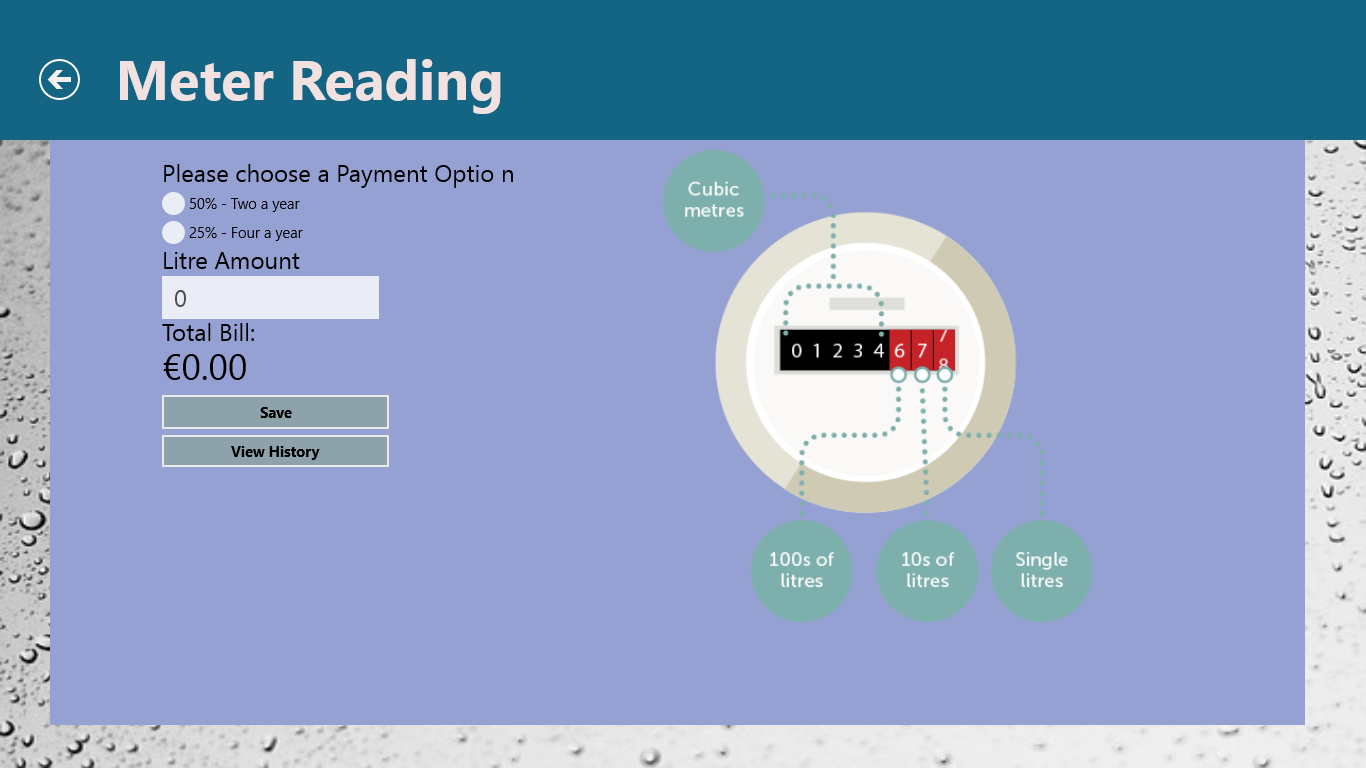
\includegraphics[scale=0.2]{ScreenShotMeterReading}

\begin{inparaenum}[]
 The main aspect to take into consideration is saving the user's information which is critical in keeping up with the user confidentiality. Using the Roaming State folder will synchronize all data on all devices which will allow the user to sign into the same account on whichever devices the user wants to log in it. This folder can be found in the AppData, Local, Packages from the Users C: drive. This allows Data sharing between the mobile application and the tablet,Desktop version. Sychronization will not happen instantly, it could depend on the device being ready to send or receive data and internet access could be another factor. Implementation of the following code creates a sampleFile.txt folder in the Roaming State on the fly and will store an object in XML format in this file.  
\end{inparaenum}

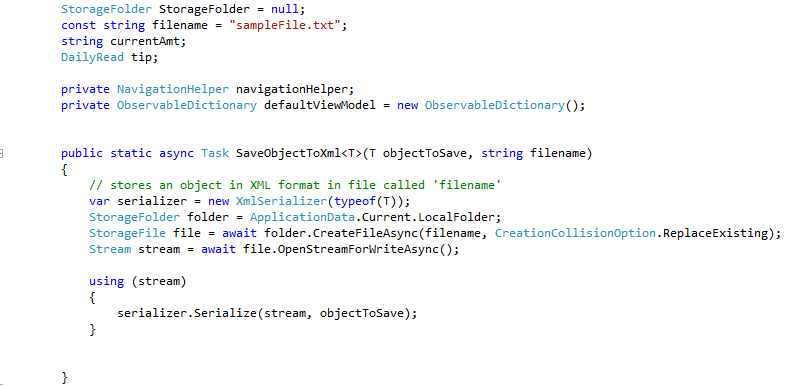
\includegraphics[scale=0.7]{RoamingCode}

This will save the meter reading total bill and litre amount to this file and allows the user to view the previous bills by clicking on the View History button. See Image 1 for reference.\\
Another useful feature is the timer which allows the user to time how long they spend using water such as taking a shower,bath and using the tap. This timer also indicates how much one single shower costs on the average of the user spending ten minutes and shows that each minute spent in the shower uses 17 litres of water. This function plays a predominant role in the user's ability to save money on their water usage. 

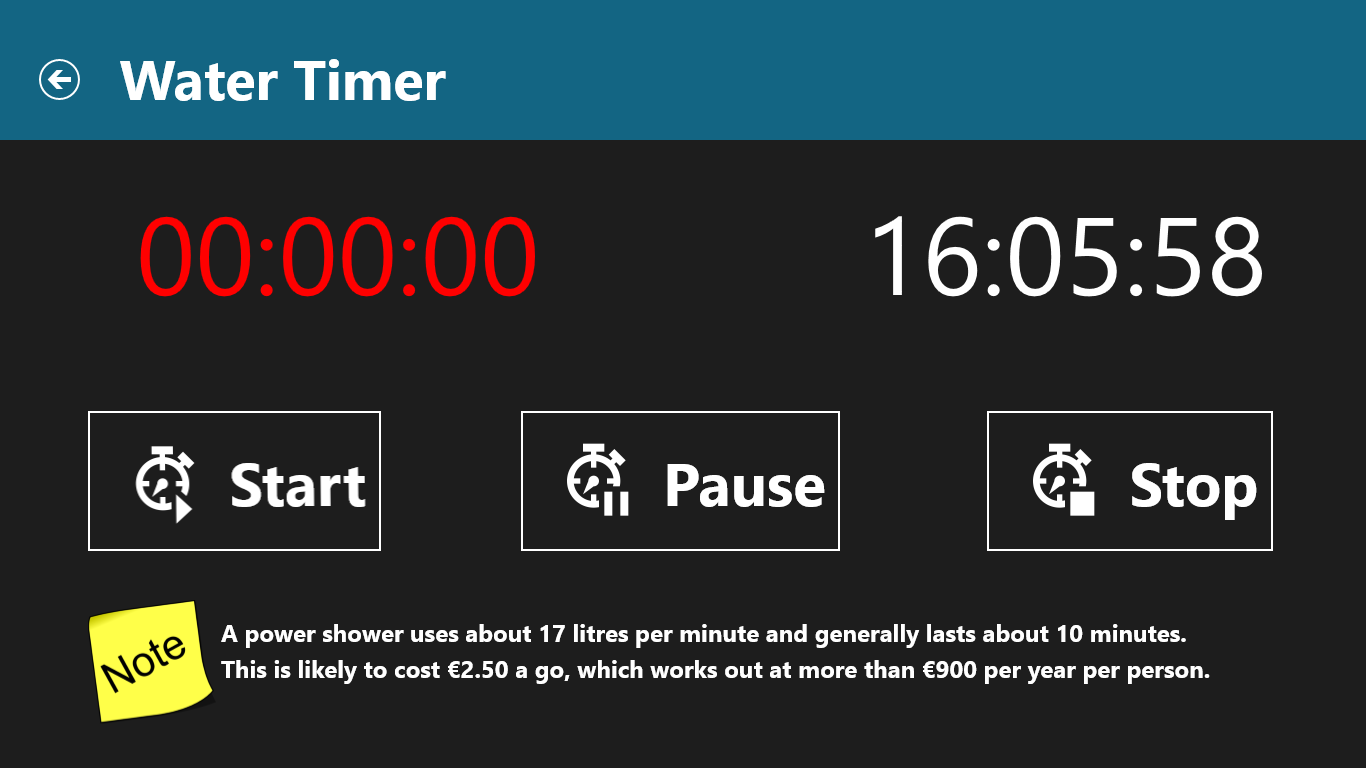
\includegraphics[scale=0.2]{ScreenShotTimer}

The system can also allow the user to create a longterm storage backup of their water meter bills by allowing them to sign in to their Onedrive account. This feature was executed by incorporating a webviewer into this page and by directing the code to the Onedrive account. See the following code snippet for reference. 

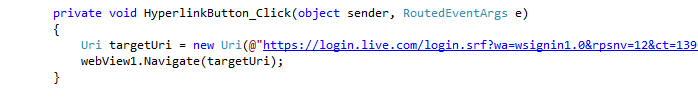
\includegraphics[scale=0.7]{OneDriveCode}

This code allows the user to click the hyperlink button and when clicked, it sends them straight to the Onedrive login page. Although the Roaming state folder stores the data longterm, this Onedrive feature gives the user a second option to manually create their own folder in their own Onedrive account to save their meter readings and bills for future use.

\includegraphics[scale=0.2]{ScreenShotOnedrive}

The system also includes a function that allows the user to create a unique account for their own use. This information is saved to the roaming folder in the AppData file, along with the bills. This is useful for the user as it uniquely identifies them and is also a good reference for the number of residents in the household as this could alter the actual water bill estimate. See image 6 for reference.

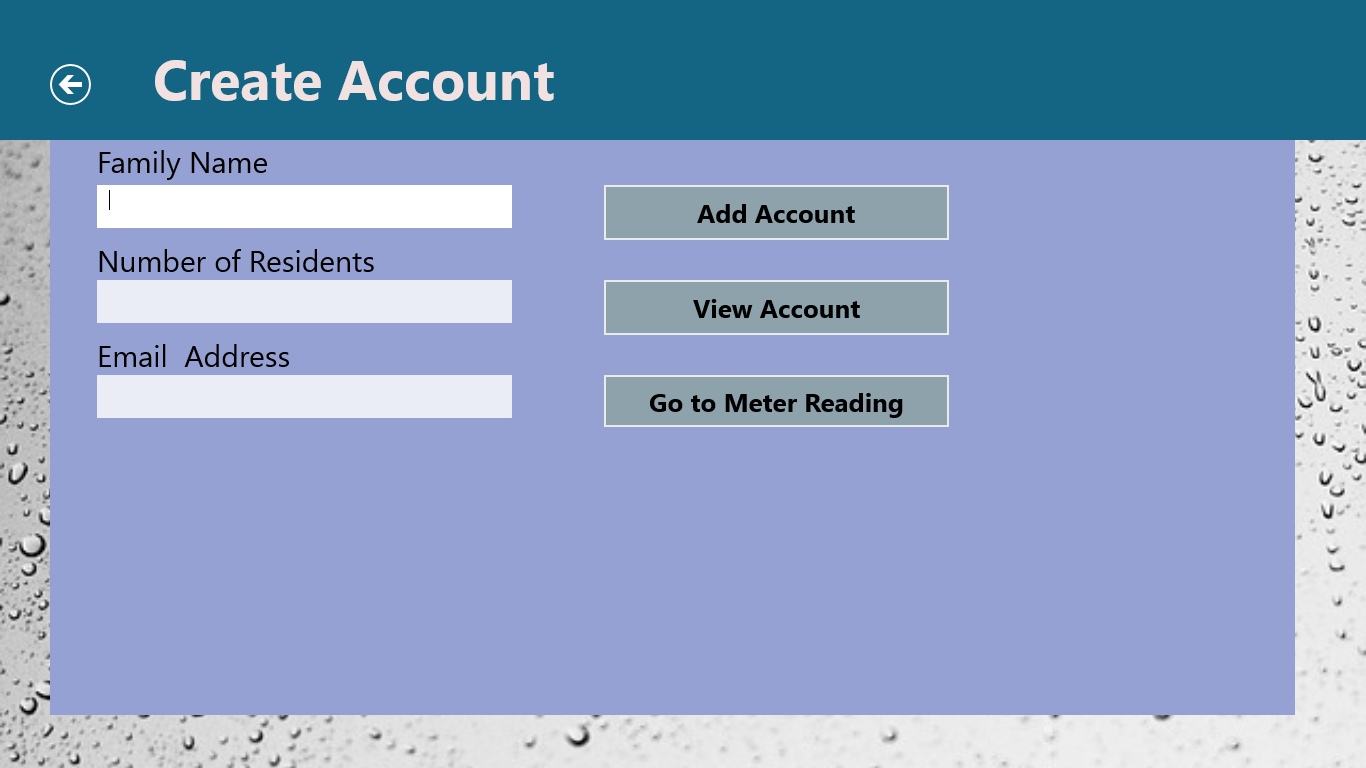
\includegraphics[scale=0.2]{ScreenShotCreate}

The application also includes two information pages, one describing detailed ways of conserving in the home and the other gives detailed estimates of how the billing system works depending on the number of residents in the household. 

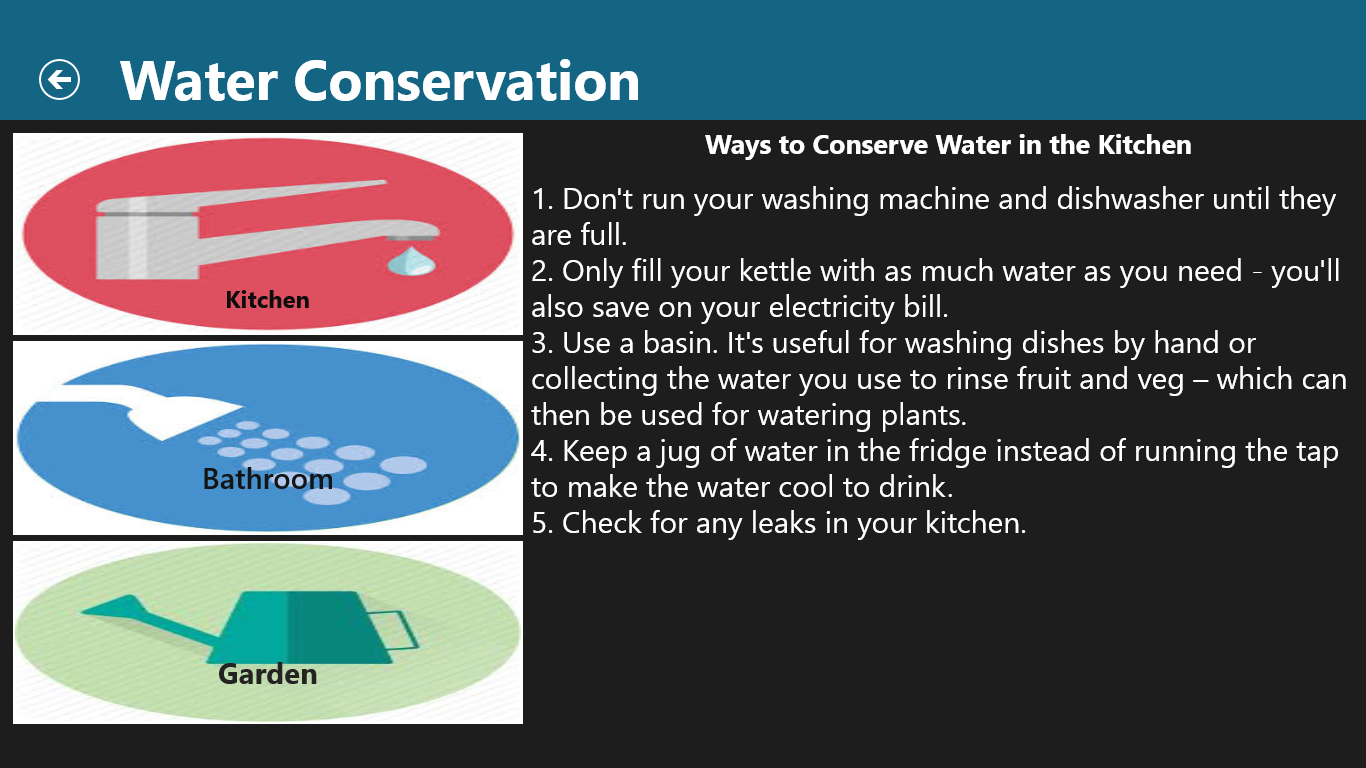
\includegraphics[scale=0.2]{ScreenShotWaterCon}

This covers all the system design and development of the tablet/desktop version of the application.

\subsection{Goal of the System Architecture}
\begin{inparaenum}[]
The major difference between the mobile phone version and tablet/desktop version of the application is the amount of data displayed. The mobile version only has four pages which includes the onedrive login, the ability to create a unique account, the meter reading calculator and the timer. The mobile phone version's main goal is to give the user the main functionality of the application without overloading them with too much information. The main reason for this is to combat the small screen size limitations with displaying more information on the tablet/desktop version of the application.
\end{inparaenum}

\section{Software Evaluation}
\label{sec:Software Evaluation}
Project planning played a predominant role in the success of the software in this application. Involvement in weekly sprints was critical in ensuring that time was well managed. Testing became a daily ritual and was a vital part of this applications software lifecycle. Once a piece of code was developed, a test was carried out to ensure its functionality was successful. When errors occurred, help was readily available. These tests gave way for major improvements in the overall performance of the application.
The main errors and failures that occurred were in the storage area of the application. Finding a storage option that would allow the user to store and view data across devices was difficult. The first option was the Live SDK API which would upload files to OneDrive only in response to an explicit user request or choice. This seemed like the ideal choice but it soon became the most difficult. The code to integrate the Live SDK API into the application was long winded and very time consuming. 
The second option was saving the data to the RoamingState folder that is found in the AppData under packages in the user account. This was found to be the best solution for saving the user's data, as it allowed the data to be saved over all devices. The code was easy to understand and once it was implemented, it create a text file on the fly where the meter bill amounts would be saved, along with the user's account information. 

\begin{inparaenum}[]
Weekly meetings with the project supervisor gave a clear indication of any errors or failures of the code. These weekly meetings also led to improvements being made to adjust the software design and architecture. Other developers opinions have also helped make some adjustments in relation to usability and design. Their opinions were greatly appreciated as it gave a feel for the different customer opinions and what type of design customers find easy to use. 
\end{inparaenum}


\section{Conclusion}
\label{sec:Conclusion}
The emergence of technology nowadays has led to a huge dependency on mobile devices. Mobile devices are now the standard for consumers when it comes to devices. They play a predominant role in people's lives on a day to day basis. People spend an average of 90 minutes per day on their mobile device, mainly on social networking sites, sending emails, blogging etc. This amount may not seem like a lot but this measures up to 23days per year of the average person's life is being spent using a smart phone. And that does not include people that spend more than 90 minutes per day on their smart phone. This can range up to 4-5hours per day, mainly for people who watch videos online,  eg. Netflix, Youtube. These statistics show how relevant this problem is, as screen size limitations effects everyone. This highlights the fact that usability is a vital part of a superior overall user experience of any application. 

\begin{inparaenum}[]
In conclusion, the overall goal of this project was to develop and design a Windows 8.1 universal application that would combat the problem of screen size limitations. The author developed and designed a user interface where a user centred approach was taken to solve the limitations of screen size on mobile devices. The amount of data displayed on the mobile version of the application is less than the amount of data displayed on the tablet/desktop version. This will alleviate the problem of the restrictions of small screen sizes, as the user has the option of viewing the list of the previous bills on the tablet/desktop version and can view the last bill on the mobile phone version. This factor contributes to a better user experience and overall superior design of the system. The mobile phone version of the application only contains four pages whereas the tablet/desktop version has six pages. The mobile phone version's main goal is to give the user the main functionality of the application without overloading users with too much information. Crystal Clear was the name chosen for this application as it has a two tier meaning. Firstly, as it represents an application to mange water bills and secondly it represents that this application is clear and concise in achieving its purpose. The developer's main aims and objectives in the development of this application were accomplished.
\end{inparaenum}

\section{Appendices}
\label{sec:Appendices}
\subsection{Installation Instructions}
1. Go to www.google.com \\
2. Search Visual Studio 2013 download.\\
3. Dreamspark is the best option if an account is available.\\
4. If Visual Studio 2012 is already on desktop then choose the update 4.\\
5. Once installed, Create shortcut to Desktop.\\
6. Then Visual Studio 2013 is ready to use.\\
		Or\\
1. Go to Windows App Store.\\
2. Search Crystal Clear.\\
3. Click install to download the application.\\

\subsection{Coding Listings}
The daily read class was implemented as follows, to perform the inside calculation of the water meter bill.
\begin{lstlisting}
// c#
using System;
using System.Collections.Generic;
using System.Linq;
using System.Text;
using System.Threading.Tasks;

namespace CrystalClearUniversal
{
    
    class DailyRead
    {
        public string FamilyName { get; set; }
        public string ResidentNo { get; set; }
        public string EmailAdd { get; set; }
        public string Date { get; set; }
        public int LitreAmount { get; set; }
        public string TipAmount { get; set; }
        public string TotalAmount { get; set; }
   
        public DailyRead()
        {
            this.FamilyName = String.Empty;
            this.ResidentNo = String.Empty;
            this.EmailAdd = String.Empty;

            this.TipAmount = String.Empty;
            this.TotalAmount = String.Empty;
        }

        public void CalculateTip(string originalAmount, double tipPercentage)
        {
            double billAmount = 0.0;
            double tipAmount = 0.0;
            double totalAmount = 0.0;

            if (double.TryParse(originalAmount.Replace('€', ' '), out billAmount))
            {

                totalAmount = (billAmount / 100) * (tipPercentage) * 3.00;

            }

            this.TipAmount = String.Format("{0:C}", tipAmount);
            this.TotalAmount = String.Format("{0:C}", totalAmount);
        }

    }
}

\end{lstlisting}

The meter reading code was implemented as follows, to store the data entered by the user.
\begin{lstlisting}
using Windows.Graphics.Display;
using Windows.Foundation.Collections;
using Windows.UI.Xaml;
using Windows.UI.Xaml.Controls;
using Windows.UI.Xaml.Controls.Primitives;
using Windows.UI.Xaml.Data;
using Windows.UI.Xaml.Input;
using Windows.UI.Xaml.Media;
using Windows.UI.Xaml.Navigation;
using Windows.Storage;
using System.Threading.Tasks;
using System.Xml.Serialization;

namespace CrystalClearUniversal
{
    public sealed partial class MeterReading : Page
    {
        List<Reading> Readings = new List<Reading>();
        StorageFolder StorageFolder = null;
        const string filename = "sampleFile.txt";
        string currentAmt;
        DailyRead tip;
        private NavigationHelper navigationHelper;
        private ObservableDictionary defaultViewModel = new ObservableDictionary();

        public ObservableDictionary DefaultViewModel
        {
            get { return this.defaultViewModel; }
        }

        public NavigationHelper NavigationHelper
        {
            get { return this.navigationHelper; }
        }

        public static async Task SaveObjectToXml<T>(T objectToSave, string filename)
        {
            // stores an object in XML format in file called 'filename'
            var serializer = new XmlSerializer(typeof(T));
            StorageFolder folder = ApplicationData.Current.LocalFolder;
            StorageFile file = await folder.CreateFileAsync(filename, CreationCollisionOption.ReplaceExisting);
            Stream stream = await file.OpenStreamForWriteAsync();

            using (stream)
            {
                serializer.Serialize(stream, objectToSave);
            }

        }

        public MeterReading()
        {
            this.InitializeComponent();
            tip = new DailyRead();
            StorageFolder = ApplicationData.Current.RoamingFolder;//will create a sampleFile.txt under the RoamingState folder

            this.navigationHelper = new NavigationHelper(this);
            this.navigationHelper.LoadState += navigationHelper_LoadState;
            this.navigationHelper.SaveState += navigationHelper_SaveState;
        }

       
        private void navigationHelper_LoadState(object sender, LoadStateEventArgs e)
        {
        }

        private void navigationHelper_SaveState(object sender, SaveStateEventArgs e)
        {
        }

        protected override void OnNavigatedTo(NavigationEventArgs e)
        {
            navigationHelper.OnNavigatedTo(e);
        }

        protected override void OnNavigatedFrom(NavigationEventArgs e)
        {
            navigationHelper.OnNavigatedFrom(e);
        }

        #endregion

        private void amountTextBox_GotFocus(object sender, RoutedEventArgs e)
        {
            billAmountTextBox.Text = "";
        }

        private void billAmountTextBox_TextChanged(object sender, TextChangedEventArgs e)
        {
            performCalculation();
        }

        private void amountTextBox_LostFocus(object sender, RoutedEventArgs e)
        {
            billAmountTextBox.Text = tip.LitreAmount.ToString();
        }
        private void performCalculation()
        {

            var selectedRadio = myStackPanel.Children.OfType<RadioButton>().FirstOrDefault(r => r.IsChecked == true);
            tip.CalculateTip(billAmountTextBox.Text, double.Parse(selectedRadio.Tag.ToString()));

            totalTextBlock.Text = tip.TipAmount;
            totalTextBlock.Text = tip.TotalAmount;
            currentAmt = tip.TotalAmount;

        }

        private void RadioButton_Click(object sender, RoutedEventArgs e)
        {
            performCalculation();
        }

        private void Save_Btn(object sender, RoutedEventArgs e)
        {
            
            WriteText(currentAmt);
            billAmountTextBox.Text = "";
            Reading reading = new Reading();
            // find day number
            reading.Day = daynum;
            DateTime now = DateTime.Now;
            string date = now.GetDateTimeFormats('d')[0];
            Readings.Add(reading);
            Save_To_XML(Readings);
        }

        private async void Save_To_XML(List<Reading> temp)
        {
            await SaveObjectToXml(temp, "Reading.xml"); 
        }

        public static async Task<T> ReadObjectFromXmlFileAsync<T>(string filename)
        {
            // this reads XML content from a file ("filename") and returns an object  from the XML
            T objectFromXml = default(T);
            var serializer = new XmlSerializer(typeof(T));
            StorageFolder folder = ApplicationData.Current.LocalFolder;
            StorageFile file = await folder.GetFileAsync(filename);
            Stream stream = await file.OpenStreamForReadAsync();
            objectFromXml = (T)serializer.Deserialize(stream);
            stream.Dispose();
            return objectFromXml;
        }

        private void View_History_Btn(object sender, RoutedEventArgs e)
        {
            ReadText();
        }

        async void ReadText()
        {
            StorageFile file = await StorageFolder.GetFileAsync(filename);
            TextBlock1.Text = await FileIO.ReadTextAsync(file);
        }
        async void WriteText(string s)
        {
            StorageFile file = await StorageFolder.GetFileAsync(filename);
            string temp = await FileIO.ReadTextAsync(file);
            temp = temp + "\n" + s;
            StorageFile writefile = await StorageFolder.CreateFileAsync(filename, CreationCollisionOption.ReplaceExisting);
            await FileIO.WriteTextAsync(writefile, temp);
          
        }

        public string daynum { get; set; }
    }
}

\end{lstlisting}

The timer was implemented with the following code, to allow the user to time the amount of time spent using water.
\begin{lstlisting}
using System;
using System.Collections.Generic;
using System.IO;
using System.Linq;
using System.Runtime.InteropServices.WindowsRuntime;
using Windows.Foundation;
using Windows.Foundation.Collections;
using Windows.UI.Xaml;
using Windows.UI.Xaml.Controls;
using Windows.UI.Xaml.Controls.Primitives;
using Windows.UI.Xaml.Data;
using Windows.UI.Xaml.Input;
using Windows.UI.Xaml.Media;
using Windows.UI.Xaml.Navigation;

namespace CrystalClearUniversal
{
    public sealed partial class Timer : Page
    {
        private DispatcherTimer timer;
        private TimeSpan timeSpan;

        public Timer()
        {
            this.InitializeComponent();
            this.timer = new DispatcherTimer { Interval = TimeSpan.FromSeconds(1) };
            this.timer.Tick += TimerOnTick;

            this.timeSpan = new TimeSpan();

            this.txtHour.Text = DateTime.Now.ToString("HH:MM:ss");
            var t = new DispatcherTimer { Interval = TimeSpan.FromSeconds(1) };
            t.Tick += (s, e) => this.txtHour.Text = DateTime.Now.ToString("HH:MM:ss");
            t.Start();
        }

        protected override void OnNavigatedTo(NavigationEventArgs e)
        {
        }

        private void TimerOnTick(object sender, object o)
        {
            this.timeSpan = this.timeSpan.Add(TimeSpan.FromSeconds(1));
            this.txtDuration.Text = this.timeSpan.ToString("c");
        }

        private void OnButtonStartClick(object sender, RoutedEventArgs e)
        {
            this.timer.Start();
        }

        private void OnButtonPauseClick(object sender, RoutedEventArgs e)
        {
            this.timer.Stop();
        }

        private void OnButtonStopClick(object sender, RoutedEventArgs e)
        {
            this.timeSpan = new TimeSpan();
            this.timer.Stop();

            this.txtDuration.Text = this.timeSpan.ToString("c");
        }

        private void backButton_Click(object sender, RoutedEventArgs e)
        {
            Frame.Navigate(typeof(MainPage));
        }
    }
}

\end{lstlisting}

The Onedrive page was generated using the following code to allow the user to access their Onedrive account.
\begin{lstlisting}
using CrystalClearUniversal.Common;
using System;
using System.Collections.Generic;
using System.IO;
using System.Linq;
using System.Runtime.InteropServices.WindowsRuntime;
using Windows.Foundation;
using Windows.Foundation.Collections;
using Windows.UI.Xaml;
using Windows.UI.Xaml.Controls;
using Windows.UI.Xaml.Controls.Primitives;
using Windows.UI.Xaml.Data;
using Windows.UI.Xaml.Input;
using Windows.UI.Xaml.Media;
using Windows.UI.Xaml.Navigation;

namespace CrystalClearUniversal
{
    public sealed partial class OneDrive : Page
    {
        private NavigationHelper navigationHelper;
        private ObservableDictionary defaultViewModel = new ObservableDictionary();

        public ObservableDictionary DefaultViewModel
        {
            get { return this.defaultViewModel; }
        }

        public NavigationHelper NavigationHelper
        {
            get { return this.navigationHelper; }
        }

        public OneDrive()
        {
            this.InitializeComponent();
            this.navigationHelper = new NavigationHelper(this);
            this.navigationHelper.LoadState += navigationHelper_LoadState;
            this.navigationHelper.SaveState += navigationHelper_SaveState;
        }

        private void navigationHelper_LoadState(object sender, LoadStateEventArgs e)
        {
        }

        private void navigationHelper_SaveState(object sender, SaveStateEventArgs e)
        {
        }

        #region NavigationHelper registration

        protected override void OnNavigatedTo(NavigationEventArgs e)
        {
            navigationHelper.OnNavigatedTo(e);
        }

        protected override void OnNavigatedFrom(NavigationEventArgs e)
        {
            navigationHelper.OnNavigatedFrom(e);
        }

        #endregion

        private void HyperlinkButton_Click(object sender, RoutedEventArgs e)
        {
            Uri targetUri = new Uri(@"https://login.live.com/login.srf?wa=wsignin1.0&rpsnv=12&ct=1396013362&rver=6.4.6456.0&wp=MBI_SSL_SHARED&wrepl");
            webView1.Navigate(targetUri);
        }

    }
}

\end{lstlisting}
The following code was implemented to generate the new account page for the user to create their unique account.
\begin{lstlisting}
using System;
using System.Collections.Generic;
using System.IO;
using System.Linq;
using System.Runtime.InteropServices.WindowsRuntime;
using Windows.Foundation;
using Windows.Foundation.Collections;
using Windows.UI.Xaml;
using Windows.UI.Xaml.Controls;
using Windows.UI.Xaml.Controls.Primitives;
using Windows.UI.Xaml.Data;
using Windows.UI.Xaml.Input;
using Windows.UI.Xaml.Media;
using Windows.UI.Xaml.Navigation;
using System.Threading;
using System.Threading.Tasks;
using Windows.Storage;

namespace CrystalClearUniversal
{
    public sealed partial class CreateAccount : Page
    {
        StorageFolder StorageFolder = null;
        const string filename = "sampleFile.txt";
        DailyRead tip;
        TimeSpan t = new TimeSpan(0, 0, 2);
        public CreateAccount()
        {
            StorageFolder = ApplicationData.Current.RoamingFolder;//will create a sampleFile.txt under the RoamingState folder.
            tip = new DailyRead();
            this.InitializeComponent();
        }

        private void Add_Account_Btn(object sender, RoutedEventArgs e)
        {
            WriteText();
        }

        private void View_Account_Btn(object sender, RoutedEventArgs e)
        {
            ReadText();
        }

        async void ReadText()
        {

            StorageFile file = await StorageFolder.GetFileAsync(filename);
            TextBlock1.Text = await FileIO.ReadTextAsync(file);

        }
        async void WriteText()
        {
            StorageFile file = await StorageFolder.CreateFileAsync(filename, CreationCollisionOption.ReplaceExisting);
            await FileIO.WriteTextAsync(file, familyNmeTxtBx.Text + "\n" + numberTxtBx.Text + "\n" + emailTxtBx.Text);
        }

        private void Go_To_MeterReading_Btn(object sender, RoutedEventArgs e)
        {
            Frame.Navigate(typeof(MeterReading));
        }

        private void backButton_Click(object sender, RoutedEventArgs e)
        {
            Frame.Navigate(typeof(MainPage));
        }
    }
}
\end{lstlisting}
The following code is implemented to generate the water conservation page which shows the user a detailed way to conserve water in three different sections in the home.
\begin{lstlisting}
using CrystalClearUniversal.Common;
using System;
using System.Collections.Generic;
using System.IO;
using System.Linq;
using System.Runtime.InteropServices.WindowsRuntime;
using Windows.Foundation;
using Windows.Foundation.Collections;
using Windows.UI.Xaml;
using Windows.UI.Xaml.Controls;
using Windows.UI.Xaml.Controls.Primitives;
using Windows.UI.Xaml.Data;
using Windows.UI.Xaml.Input;
using Windows.UI.Xaml.Media;
using Windows.UI.Xaml.Navigation;

namespace CrystalClearUniversal
{
    public sealed partial class WaterConservation : Page
    {

        private NavigationHelper navigationHelper;
        private ObservableDictionary defaultViewModel = new ObservableDictionary();

        public ObservableDictionary DefaultViewModel
        {
            get { return this.defaultViewModel; }
        }

        public NavigationHelper NavigationHelper
        {
            get { return this.navigationHelper; }
        }


        public WaterConservation()
        {
            this.InitializeComponent();
            this.navigationHelper = new NavigationHelper(this);
            this.navigationHelper.LoadState += navigationHelper_LoadState;
            this.navigationHelper.SaveState += navigationHelper_SaveState;
        }

        private void navigationHelper_LoadState(object sender, LoadStateEventArgs e)
        {
        }

        private void navigationHelper_SaveState(object sender, SaveStateEventArgs e)
        {
        }

        #region NavigationHelper registration

        protected override void OnNavigatedTo(NavigationEventArgs e)
        {
            navigationHelper.OnNavigatedTo(e);
        }

        protected override void OnNavigatedFrom(NavigationEventArgs e)
        {
            navigationHelper.OnNavigatedFrom(e);
        }

        #endregion

        private void kitchen_Click(object sender, RoutedEventArgs e)
        {
            this.txtInformationKitchen.Visibility = Visibility.Visible;
            this.txtInformationBathroom.Visibility = Visibility.Collapsed;
            this.txtInformationGarden.Visibility = Visibility.Collapsed;

            this.txtKitchenInfo.Visibility = Visibility.Visible;
            this.txtBathInfo.Visibility = Visibility.Collapsed;
            this.txtInfoGarden.Visibility = Visibility.Collapsed;
        }

        private void bathroom_Click(object sender, RoutedEventArgs e)
        {
            this.txtInformationBathroom.Visibility = Visibility.Visible;
            this.txtInformationKitchen.Visibility = Visibility.Collapsed;
            this.txtInformationGarden.Visibility = Visibility.Collapsed;

            this.txtKitchenInfo.Visibility = Visibility.Collapsed;
            this.txtBathInfo.Visibility = Visibility.Visible;
            this.txtInfoGarden.Visibility = Visibility.Collapsed;
        }

        private void garden_Click(object sender, RoutedEventArgs e)
        {
            this.txtInformationGarden.Visibility = Visibility.Visible;
            this.txtInformationKitchen.Visibility = Visibility.Collapsed;
            this.txtInformationBathroom.Visibility = Visibility.Collapsed;

            this.txtKitchenInfo.Visibility = Visibility.Collapsed;
            this.txtBathInfo.Visibility = Visibility.Collapsed;
            this.txtInfoGarden.Visibility = Visibility.Visible;
        }
    }
}
\end{lstlisting}


\bibliographystyle{plainnat}
\bibliography{LitBibTech}

\end{document}


